\chapter{Temporal network analysis}
The previous chapter has demonstrated that network analysis provides a deep insight into the processes behind epidemic spreading.
Given a sufficient amount of data, a contact network is capable to capture all possible infection pathways in the system.
The potential of static network analysis lies in the huge toolbox of methods that has been developed in the last decades.
As depicted in section \ref{sec:network_theory}, there exist coherent definitions for both their large scale topological features and local centrality measures allowing for node rankings.

Nevertheless, the concept of static networks neglects temporal variations in the system, i.e. the edges of a particular network are not necessarily present all the time.
This chapter addresses some of the conceptional problems owing to a sparse and heterogenous occurrence of edges in the network, the most central one being the \emph{causality of paths} in the network.
Section \ref{sec:Plos} focusses on the computational analysis of the full temporal representation of the network analyzed (from the static perspective) in section \ref{sec:network_analysis}.
In section \ref{sec:PRL}, we present a novel formalism mapping the causality of temporal networks onto a mathematical graph.

\section{Introduction}
To begin with, we highlight the most fundamental difference between static and temporal networks.
In particular, we compare the static and the temporal representation of the system.
Figure \ref{fig:temporal_network_principle} shows a temporal network and its aggregated graph.
%
\begin{figure}[htb]
\begin{center}
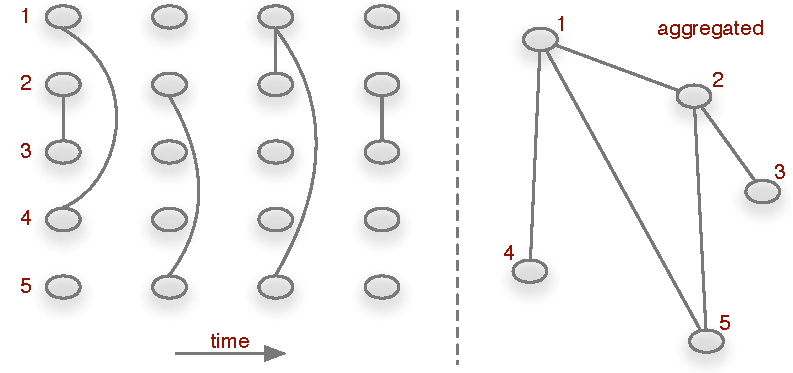
\includegraphics{Temporal_Network_Principle.pdf}
\caption{%
Role of causality in a temporal network with $5$ nodes and $4$ snapshots.
The left panel shows snapshots of the system at different times and the right panel shows the corresponding aggregated network.
Although there is a path from node $3$ to $4$ (and vice versa) in the aggregated network (right panel), there is no causal path between $3$ and $4$ in the temporal network (left panel).
}
\label{fig:temporal_network_principle}
\end{center}
\end{figure}
%
Although the edges of the temporal network are present in the aggregated graph, the situation becomes more complex, if we consider paths of length greater than one.
The aggregated graph (right panel in figure \ref{fig:temporal_network_principle}) suggests that the network is connected, i.e. there is a path between every node pair.
As an example, there are two different paths from node $3$ to $4$ in the aggregated system.
However, this does not hold for the temporal system.
Consequently, paths in an aggregated graph of a temporal network have to be treated with care.

Before we give a formal definition of temporal networks, we have to distinguish between terms used for temporal networks and other systems.

\paragraph{Disambiguation\color{Cayenne}{.}}
Since the analysis of temporal networks is an interdisciplinary field, there is still no consistent designation for what the author refers to as \emph{temporal networks} \citep{Holme_review}.
Different phrases, such as temporal graphs, dynamic graphs, dynamic networks are used in the literature.
In addition to that, there are other classes of networks seeming to be related to temporal networks, i.e. adaptive networks, growing networks, evolving graphs.
The analysis of the latter has a strong focus on network growth, i.e. the process behind the evolution of static networks.
A central question for these systems is what is the fundamental process that has formed the network.
An example is the \BA network, where the underlying process is a rich-get-richer principle that results in a scale free degree distribution.
The striking difference between growing networks and temporal networks is that the snapshots of a temporal network can in principle be arbitrary.
Correlations between two snapshots of the system (if any) could be over arbitrary periods of time.
We prefer the term temporal network, since \emph{temporal} is not so easily confused with dynamic systems.
Furthermore, the systems under consideration are not mathematical graphs; therefore, we use the more general term \emph{network}.

\paragraph{Formal definition\color{Cayenne}{.}}
A temporal network $\mathcal{G}=(V,\mathcal{E},T)$ consists of a set of nodes $V$ and a set of edges $\mathcal{E}$, where each edge in $\mathcal{E}$ is given by a triple $(u,v,t)$ and connects nodes $u$ and $v$ at time $t\in T$.
$T$ is the observation period of $\mathcal{G}$, where $T\subset \mathbb{N}^+$ for time discrete systems and $T\subset \mathbb{R}^+$ for continuous systems.
\footnote{
In this work, we focus on time discrete systems, since a continuous time process can be approximated by a discrete one by choosing an appropriately small increment.
Furthermore, edge weights and a latency functions for edge traversal could be added to the definition \citep{Casteights_review}.
This is, however, beyond the scope of this thesis.
}
The aggregated graph $G=(V,E)$ of a temporal network simply ignores the occurrence times of the edges in $\mathcal{E}$ and the set of nodes $V$ is the same in both representations.

\paragraph{Viewpoints and implementation\color{Cayenne}{.}}
As in the case of static networks, temporal networks can be interpreted and implemented in different ways \citep{Casteights_review}.
A brief report of different implementations of static networks is given in Appendix \ref{sec:implementation}.
Besides the adjacency matrix, edge lists and adjacency lists are appropriate network representations.
Considering a temporal network as a sequence of static networks (called snapshots or graphlets) can be seen as a \emph{graph centric} view on the system.
It is the analogue of the adjacency matrix in static networks.
More formally, a temporal network $\mathcal{G}$ is represented by a sequence of adjacency matrices
\begin{equation}\label{eq:AdMatrixSequence}
\mathcal{A}=\mat{A}_1,\dots ,\mat{A}_T,
\end{equation}
where $T$ is the observation time and the increment is the temporal resolution.

In analogy to the edge lists of static networks (see Appendix \ref{sec:implementation}), an \emph{edge centric} view on a temporal network consists of the occurrence times of the edges.
Let $\mathcal{G}=(V,\mathcal{E})$ be a temporal network.
Than the set of edges $\mathcal{E}$ is represented by a sequence of triples
\begin{equation*}%\label{eq:temporal_edges}
\mathcal{E}=(u_1,v_1,t_1),(u_1,v_1,t_2),(u_2,v_2,t_2),\dots \;.
\end{equation*}
An edge centric view focusses on the occurrence times of each edge, i.e.
\[
\mathcal{I}((u_1,v_1))=t_2,t_2,\dots \; .
\]
This point of view is particularly convenient for the time randomization of temporal networks (see section \ref{sec:randomized_models_tvg}).
Finally, a \emph{node centric} view of a temporal network considers the neighborhood $\mathcal{N}$ of a node $v$ over time, i.e. $\mathcal{N}(v,t)$.
This view corresponds to the adjacency list of a static network (see Appendix \ref{sec:implementation}).
The temporal degree of each node immediately follows from $d(v,t)=\abs{\mathcal{N}(v,t)}$.
The edge centric and node centric network view is considered as a microscopic perspective, while the graph centric view provides a macroscopic perspective.

We make use of microscopic perspective implicitly in computer implementations as in section \ref{sec:Plos}.
Furthermore, we focus on the graph centric view \eqref{eq:AdMatrixSequence} in section \ref{sec:PRL} to analyze macroscopic path structures in temporal networks.

\paragraph{Paths in temporal networks\color{Cayenne}{.}}
A causal sequence of edges between two nodes $u$ and $v$ in a temporal network is called (causal) path.
It is given by a sequence of edges, i.e.
\[
\mathrm{path}(u,v,t)= \{ (u,x,t_1),(x,y,t_2),\dots ,(z,v,t_n) \}, 
\]
where $ t_1<t_2<\dots <t_n$ and $x$, $y$ and $z$ are nodes on the path.
%
\begin{SCfigure}
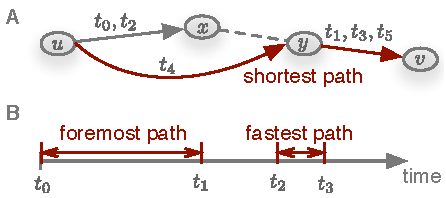
\includegraphics{Shortest_foremost_fastest.pdf}
\caption{Topological shortest distance and temporal shortest durations for a path between nodes $u$ and $v$.
The shortest path (panel A) counts the number of edges between the nodes.
Panel~B demonstrates that although the fastest path could take $t_3-t_2 < t_1-t_0$, the foremost path arrives already at $t_1<t_2$.
}
\label{fig:shortest_foremost_fastest}
\end{SCfigure}

Note that possible paths between nodes depend on time in general.
This has crucial implications on the \emph{shortest path distance} known from static networks (see section  \ref{sec:network_terminology}).
As a matter of fact, there are three different shortest path types in temporal networks.
Just like in the static case, the shortest path distance between two nodes measures the topological distance between the nodes.
It counts the number of edges used do traverse the shortest path.
In addition, the \emph{duration} of a path can be measured in temporal networks.
This duration can be measured in two different time frames \citep{Casteights_review}:
First, the \emph{fastest} path between two nodes is the path of shortest duration, no matter when the path starts in time.
Second, the \emph{foremost} path between two nodes is the path that arrives earliest in a global time frame.

Figure \ref{fig:shortest_foremost_fastest} demonstrates the difference between the foremost, fastest and shortest path concept, respectively.
Edge labels are edge occurrence times, which are ordered so that $t_1<t_2<t_3<t_4<t_5$.
The dashed edge $(x,y)$ indicates that these nodes are not connected directly, but by other nodes of the network.
Panel A shows that the shortest topological path between nodes $u$ and $v$ is $(u,x,v)$ and the distance is $3$.
It can be seen from panel B that the first (foremost) path start at node $u$ at time $t_0$ and arrives at node $v$ at time $t_1$.
Although the fastest path takes less time to traverse ($t_3-t_2<t_1-t_0$), it arrives later ($t_3>t_1$) than the foremost path.
Note that shortest path and temporal shortest path do not coincide in this example, since the shortest path connection can be at times $t_4$ and $t_5$ which are greater than $t_1$ and $t_3$.

Throughout the rest of this work, we use a global time scale, which is defined by the first time in the dataset under consideration.
Consequently, we measure shortest path durations in terms of \emph{foremost} path durations, if not explicitly stated.

\subsection{Conceptual problems in temporal networks}\label{sec:conceptual_problems}
Before we focus on different methods to analyze temporal networks, we have to point out that many static network measures, such as centrality or components, are in general time-dependent and can not be summarized to single numbers.
In addition, time-scales of node dynamics and network dynamics can be of the same order and cause significant interactions between the dynamics.



\section{Data driven network analysis}\label{sec:Plos}
In this section we analyze the pig trade data set as introduced in section \ref{sec:network_analysis}, but we explicitly take into account temporal information%
\footnote{%
In order to be congruent with the datasets used in the publications, we use the pig trade dataset of \citep{Konschake:2013js} in this chapter.
This dataset differs slightly from the dataset used in section \ref{sec:network_analysis}.
It covers the period from 01 January 2008 to 31 December 2009.
The results do not change qualitatively and hereby the results of \citep{Konschake:2013js} and \citep{Lentz:2013PRL} are comparable.}. %
Each edge in the system is only present at certain days.
Long waiting times between edge occurrences can be present in the system.

As in the case of static networks, the concept of centrality plays an important role for risk assessment and the implementation of vaccination and surveillance strategies also in time-varying topologies.
The maximum spreading potential of each node is given by its range as discussed for static networks in section \ref{sec:network_analysis}.
In this section we analyze the out-component of the network nodes according to their constance over time.

\subsection{Representative sample}
Before we analyze the ranges of the nodes in the network, we estimate the time span needed to cover the temporal properties of the system.
Figure \ref{fig:Plos_S1} A shows the activity of the nodes and edges in the network over the observation period.
The red line shows the number of active nodes on a daily resolution.
We observe that 25~\% of all nodes and 10~\% edges are active every day on average.
The plot shows decreased activity during the summer month and on public holidays such as easter and christmas.
In addition, there is a slight trend to a decrease of the number of nodes, which reflects a centralizing process in the system.
%
\begin{figure}[htbp]
\begin{center}
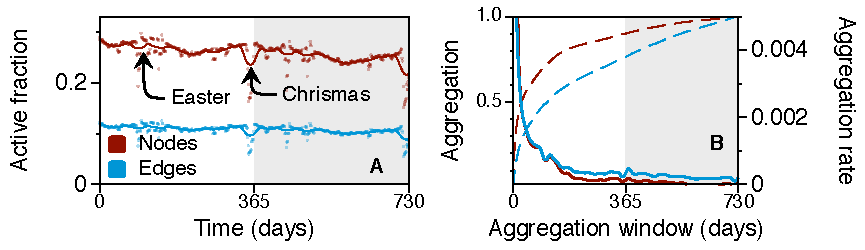
\includegraphics{Plos_S2AB.pdf}
\caption{\textbf{Panel A:} Daily activity of the network over two years.
Original data is shown as points and solid lines are local regressions of the original data.\\
\textbf{Panel B:} Time aggregation of the network for different aggregation windows.
Dashed lines show the fractions of nodes/edges in the aggregated network.
Solid lines are local regressions of the aggregation rates.
}
\label{fig:Plos_S1}
\end{center}
\end{figure}

Figure \ref{fig:Plos_S1} B gives a picture of the convergence of the network during the aggregation process, i.e. summing up the snapshots of the temporal system to obtain the static network representation.
The network is successively aggregated over more and more snapshots.
Dashed lines show the fractions of nodes and edges in the aggregated network, respectively.
The solid lines show the respective aggregation rates.
Since the latter are derivatives of the aggregation fractions, we do show a local regression of the aggregation rate to reduce noise in the signal.

The figure demonstrates that the aggregation rates for both nodes and edges becomes negligible after 1 year.
Therefore, we can assess a period of 1 year sufficient to provide stationarity of the system, i.e. the time span, after which only few more edges are added to the network.

\subsection{Simulated disease outbreaks}
Node rankings are of major importance for epidemiology.
We try to answer the question, if a constant ranking of node makes sense on a temporal network.
As a generic measure for the spreading potential of a node, we consider the range.
In analogy to section \ref{sec:network_analysis}, we define the range of a node in a temporal network as the size of its temporal out-component.
It is important to note that the out-component of each node depends on the time $t_0$, when it is measured.
Additionally, an epidemic taking place on the network can have a finite infectious period $k$, i.e. a time period, after the infection dies out if it is not carried over to another agent.
This mimics an SIR-type process, where the infectious period is given by the reciprocal recovery rate (see section \ref{sec:sir_model}).
More generally, $k$ corresponds to the memory of a process taking place on the network.
This process could be a chemical reaction or rumor spread.

For clarity reasons we do not solve differential equations for epidemics in this section and reduce the infection dynamics to assigning a discrete infection state -- susceptible, infected or recovered -- to each node in the network (see section \ref{sec:epi_networks}).
An infected node remains infected over the infectious period $k$.
We define the \emph{temporal range} of a node $v$ by explicitly taking into account the time of (primary) infection and infectious period, i.e.
$r_v (k,t_0)$.
Since there are no mixing states of nodes as in mate populations and we assume an infection probability $p=1$, the range of a node is identical to the outbreak size. 

\subsubsection{Single outbreaks}
We discuss the outbreak pattern caused by single outbreaks in this section, while we discuss the properties of the ensemble of all possible outbreak scenarios in the next section.
In order to analyze node ranges in the pig trade network, we use a modified breadth-first-search algorithm (see Appendix \ref{sec:implementation} for a brief summary of search algorithms for static networks).
Given a fixed infectious period, we mark a particular node $v$ to be infected at time $t_0$.
For every time step in the interval $[t_0,t_0+k]$, we identify the neighborhood $\mathcal{N}(v,t)$ and mark all susceptible nodes in $\mathcal{N}(v,t)$ as infected.
Infected nodes are marked as removed after the infectious period $k$ and do not contribute to further infections.
This procedure is repeated for all infected nodes as long as there are still infected nodes in the system.

\begin{SCfigure}
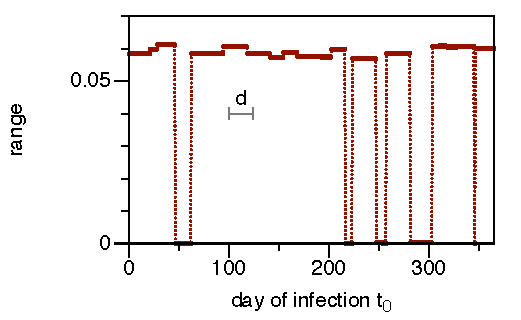
\includegraphics{exemplary_range.pdf}
\caption{Temporal variation in the range $r_v(k,t_0)$ of an exemplary node $v$ in the network over one year.
Although the range remains rather constant for most infection times, it vanishes for certain periods.
The grey interval corresponds to the fixed infectious period $k=24$~days.
}
\label{fig:range_exemplary}
\end{SCfigure}
%
Figure \ref{fig:range_exemplary} shows the range of an exemplary node in the network for different infection times $t_0$.
The infectious period is $k=24$ days.
For most infection times the example node can infect about $6~\%$ of the network.
The range distribution shows a similar bimodal pattern as already seen for the static network in figure \ref{fig:node_range}.
This provides evidence that there is an infection path from the exemplary node to a connected component in the network.
It is important to stress that the concept of connected components does not translate to temporal networks in a straightforward manner (see section \ref{sec:conceptual_problems}).
Besides the bimodality itself, it remarkable that the majority of adjacent primary infection times cause outbreaks of similar size.

This feature is can be explained, if we underline the temporal sparsity of edges, i.e. nodes are likely to have only few contacts within one infectious period.
If the primarily infected node $v$ has no trade contact within the infectious period, the disease dies out.
Even if the disease is transferred to a successor node $w$ at a time $t_1$ within the interval $[t_0,t_0+k]$, the disease dies out, if there is not further trade contact within the period $[t_1+k]$ and so forth.
The regions of small/vanishing range in figure \ref{fig:range_exemplary} correspond to these scenarios.
On the other hand, if all successors of node $v$ have 1 or more trading contacts within their respective infectious periods, the disease can be transferred to a larger number of nodes.
The majority of small variations in $t_0$ implies stable ranges in the order of $k$ (the infectious period is shown by the grey line in figure \ref{fig:range_exemplary}).
If the degree of $v$ or a successor node in the infection chain is even larger than 1, even more secondary outbreaks are triggered and manifest themselves in smaller range fluctuations as for the long range values in \ref{fig:range_exemplary}.

We have seen in this section that a temporal degree of freedom adds a significant amount of complexity even to the outbreak pattern of a single node.
Now we focus on the ensemble of all outbreak scenarios, i.e. the ensemble of all initial conditions and variations in the infectious period as a parameter.
%
\subsubsection{Outbreak ensemble}
We apply the method discussed in the previous section to all nodes in the network.
As primary infection times, we consider all times within the first year in the dataset.
This ensures that even if a particular outbreak penetrates the second year, it will have died out within the observation period.
We restrict ourselves to infectious periods $k<56$~days, since this interval covers the infectious periods of the major livestock diseases \citep{Horst:1998wu,Konschake:2013js}.
Considering all nodes in the network as potential starting points for infections and all days in the first year of the dataset as possible starting times yields $10^9$ different initial conditions.
We denote the \emph{ensemble of all outbreak scenarios} by $\mathcal{S}$.
More formally, let $\mathcal{G}=(V,\mathcal{E},T)$ be the temporal network of our dataset.
Then the ensemble of all outbreaks is given by all possible initial conditions and parameters and the corresponding outbreak size, where the latter is identical to the range for our model:
\begin{equation}\label{eq:outbreak_ensemble}
\mathcal{S}=\left\{ (v,t_0,k,r_v(k,t_0)): v \in V,t_0 \in T/2, k \leq 56  \right\}.
\end{equation}

In static networks, every node can cause an epidemic, if it is connected to other nodes in the network.
We have seen in the previous section that the time of primary infection has to be in an appropriate interval in temporal networks.
In addition, this constraint depends on the infectious period, since a disease with high infectious period is more likely to spread over the network than a disease with low infectious period.
Figure \ref{fig:plosfig1} A shows the outbreak probability for different infectious periods.
The outbreak probability (solid line) is measured as the fraction of elements in $\mathcal{S}$ that causes a secondary outbreak at all.
For comparison, the outbreak probability in the static network is shown as dashed.
This is just the fraction of nodes with finite out degree and apparently the outbreak probability shows no dependence on the infectious period in the static case.
The outbreak probability saturates for sufficiently large infectious periods, but it is still only half as much as in the static case even for $k=56$.
%
\begin{figure}[htbp]
\begin{center}
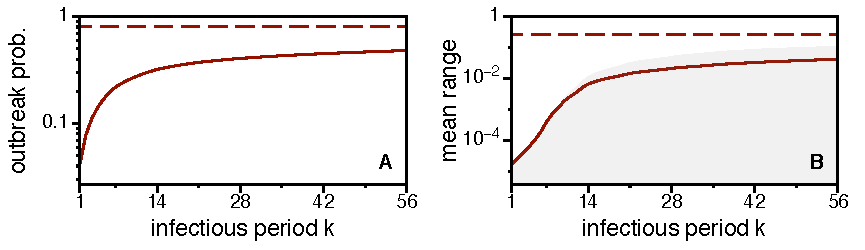
\includegraphics{Plos_fig1}
\caption{Outbreak probability (A) and mean range (B) for different infectious periods $k$ as solid lines.
Dashed lines correspond outbreak probability and mean outbreak size of the static network, respectively.
The grey shaded area in panel B shows the 50~\% confidence interval.}
\label{fig:plosfig1}
\end{center}
\end{figure}

In addition to the probability of an outbreak, we compute the expected size of the outbreaks.
The mean outbreak size is an average over all starting nodes and all starting times in $\mathcal{S}$.
Figure \ref{fig:plosfig1} B shows the mean outbreak size and the 50~\% confidence interval (solid line and grey shaded area) and the mean outbreak size in the static network (dashed line).
As for the outbreak probability, we observe significant outbreak sizes only for $k>14$~days and the outbreak size is 6 times smaller than in the static case even for $k=56$~days.
In summary, the infectious period must be larger than 14~days to cause a severe outbreak and the static network approximation overestimates the size of outbreaks significantly.

\subsection{Node rankings}
This section is devoted to the analysis of the node ranking according to their respective ranges.
For every infectious period $k$, we average over all times of primary infection in the ensemble $\mathcal{S}$ \eqref{eq:outbreak_ensemble}.
This gives a ranking $R(k)$ of the nodes according to their outbreak sizes.
The question here is, whether these rankings remain stable, if the infectious period is changed.
%
\begin{SCfigure}
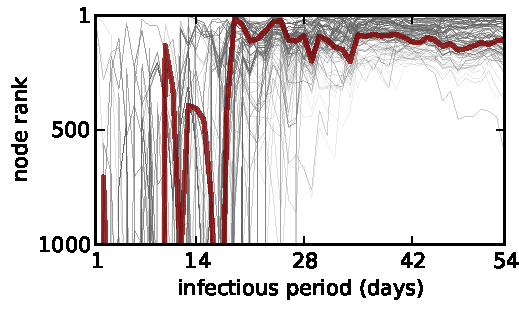
\includegraphics{vir_ranking.pdf}
\caption{Node ranking of the top 100 nodes over different infectious periods.
Rankings are computed by averaging \eqref{eq:outbreak_ensemble} over the time of primary infection.
Top 100 nodes are the nodes with the largest outbreak sizes averaged over $k$ and $t_0$.
The rankings of an arbitrary node are shown in red for illustration purposes.}
\label{fig:ranking}
\end{SCfigure}

Figure \ref{fig:ranking} shows the ranking trajectories over different infectious periods of the top 100 nodes in the network. 
We define the top 100 nodes as the nodes with the largest outbreak size in $\mathcal{S}$ averaged over both $t_0$ and $k$.
An arbitrarily chosen node is shown in red for illustration purposes.
It should be noted that the rank of each node in the top 100 set can take any value in the figure, since the top 100 nodes are determined by averaging out the infectious period.

As the figure suggests, the ranking of nodes is unstable for small infectious periods ($k<21$~days).
This region is dominated by temporal fluctuations of the infection paths in the network.
Interestingly, the ranking approaches a stable region for $k>21$~days.
For $k>28$~days most nodes in the top 100 sample do not undergo significant rank changes any more.
This means that a ranking of nodes is reasonable for sufficiently large infectious periods.


\paragraph{Correlations vs. Intersections\color{Cayenne}{.}}


\subsection{Temporal vs. static representation}

\section{Graph centric temporal network analysis}\label{sec:PRL}

\subsection{Matrices for temporal networks}

\subsection{Representative sample / characteristic time scale}

\subsection{Causal fidelity}

\subsection{Temporal and topological mixing patterns}

\subsection{Randomized models}\label{sec:randomized_models_tvg}





